\Chapter{Core Concepts and Previous Research}

\Section{Fuzzy Logic}
In order to gain a sound understanding of the idea of \textit{fuzziness} we must first familiarize ourselves with the notion of fuzzy sets. The concept was first introduced and described by mathematician Lotfi A. Zadeh in 1965 as an extension to classical sets. The key difference between ordinary sets and fuzzy ones is simple: In the case of the former all elements are either a part of a set or not, where as in the world of fuzzy sets an element may belong to multiple sets. The measure of how much an element is part of a given set is referred to as its \textit{degree of membership} and is calculated with the aid of the \textit{membership function}.

\SubSection{Fuzzy Set}
As opposed to classical sets, every element in a fuzyz set has an additional property beside its value that being the degree to which that given element is the set. These aspects are more formally defined in the following section.

\begin{definition}
Let $U$, referred to as the \textit{universe of discourse}, be a set containing all the elements we wish to describe and define $m:U \to [0, 1]$ as a membership function. The pair $(U, m) $ forms a fuzzy set $A$ in which $\forall x \in U$ the value given by $m(x)$ is called the degree of membership of $x$. The function $m(x)$ is equivalent to $\mu_{a}(x)$.
\end{definition}

Taking the example from Claudio Moraga's \textit{Introduction to fuzzy logic} (2005) \cite{moraga2005}: given the interval $[0, 10]$ of the real line as our universe of discourse and the statement ``x is between 3 and 5'', we may represent it with the function $\mu_{3-5}:[0, 10] \to [0,1]$. Where $\mu_{3-5}(x) = 1$ if $3 \leq x \geq 5$, and $\mu_{3-5}(x) = 0$ otherwise as seen on fig1.a. This function describes the classical set $[3, 5]$. Consider now the statement ``x is near 4''. The proximity, or nearness to the number $4$ can be represented as $4-\epsilon$, given the assumption that $\epsilon$ is a sufficiently small positive real number. Values obtained by the continued subtraction of $\epsilon$ will have a decreasing \textit{``degree of nearness''} to $4$ until the value, and subsequently those smaller then itself, is no longer considered to be ``near'' the number $4$. Repeating this experiment with $4+\epsilon$ and the continued addition of $\epsilon$ will yield symmetric results. If we take the function $\mu_{near 4} : [0, 10] \to [0, 1]$ to represent this statement just as previously, it becomes apparent that it cannot be of the same kind as $\mu_{3-5}$ (that lead to a classical set). If we assume that 3 and 5 are acceptable limit points for ``near 4” and marking these as , $\alpha_{min} = 3, \alpha_{max} = 5, beta = 4$, then

\[
	\mu_{near 4}(x) =
		\begin{cases}
			0, &x \leq \alpha_{min} \text{ or } x \geq \alpha_{max}\\
			1, &x = \beta\\
			\frac{x - \alpha_{min}}{\beta - \alpha_{min}}, &\alpha_{min} < x < \beta\\
			\frac{\alpha_{max} - x}{\alpha_{max} - \beta}, &\beta < x < \alpha_{max}.\\
		\end{cases}
\]

The function will be continuous and increasing for $3 < x < 4 and$ will be continuous and decreasing for$ 4 < x < 5$. Without further information, linear transitions will be chosen as shown in fig1.b. $\mu_{near 4} $ represents a \textbf{fuzzy set}.

[figures of the previous example]
\begin{figure}[!h]
\centering
\begin{subfigure}{.5\textwidth}
	\centering
	\begin{tikzpicture}
		\draw (-3, 0) -- (3, 0);
		\draw (-3, 0) -- (-3, 3);
		\draw (-3, 3) -- (3, 3);
		\draw (3, 0) -- (3, 3);
 	\end{tikzpicture}
  	\caption{Classical set}
  	\label{fig:sub1}
\end{subfigure}%
\begin{subfigure}{.5\textwidth}
	\centering
  	\begin{tikzpicture}
		\draw (-3, 0) -- (3, 0);
		\draw (-3, 0) -- (-3, 3);
		\draw (-3, 3) -- (3, 3);
		\draw (3, 0) -- (3, 3);
	\end{tikzpicture}
  	\caption{Fuzzy set}
  	\label{fig:sub2}
\end{subfigure}
\caption{Difference in steepness during the transition from 0 to 1.}
\label{fig:steepness}
\end{figure}

Other than assigning values linearly to elements not fully contained inside a fuzzy set any kind of membership function can be utilized, but by far the most common is the previously mentioned linear way, which produces a trapeziod shape during visualization (Triangles arise, when the upper side of the trapezoid is a point). As mentioned by \cite{sabri2013}, in terms of terminology the following expressions are defined regarding any given fuzzy set:

\textit{Core:} Elements where the membership function is 1:
\[
	\text{core}(A) = \{x \in U \vert \mu_{\alpha}(x) \geq \alpha\}
\]

\textit{Support:} Elements where the membership function is greater than 0:
\[
	\text{support}(A) = \{x \in U \vert \mu_{\alpha}(x) > 0\}
\]

\textit{Boundary:} Elements where the membership function is between 0 and 1:
\[
	\text{boundary}(A) = \{x \in U \vert 0 < \mu_{\alpha}(x) < 1\}
\]

\textit{Height:} The height of the fuzzy set $A$ is the maximum value taken on by the membership function:
\[
	\text{height}(A) = \{x \in U \vert \max(\mu_{\alpha}(x))\}
\]

\SubSection{Various Membership Functions}
An example of the different shapes that a membership function may take include the following cases and their respective definitions appearing in \cite{sabri2013}:

\textbf{Triangular} (Same as in the above example, a special case of the trapezoid):
\[
	\mu_{A}(x) =
		\begin{cases}
			0, &x \leq \alpha_{min} \text{ or } x \geq \alpha_{max}\\
			1, &x = \beta\\
			\frac{x - \alpha_{min}}{\beta - \alpha_{min}}, &\alpha_{min} < x < \beta\\
			\frac{\alpha_{max} - x}{\alpha_{max} - \beta}, &\beta < x < \alpha_{max}.\\
		\end{cases}
\]

\textbf{Trapezoidal} (With the upper side (core) taking values from [$\beta_1$, $\beta_2$]):
\[
	\mu_{A}(x) =
		\begin{cases}
			0, &x \leq \alpha_{min} \text{ or } x \geq \alpha_{max}\\
			\frac{x - \alpha_{min}}{\beta_1 - \alpha_{min}}, &\alpha_{min} < x < \beta_1\\
			\frac{\alpha_{max} - x}{\alpha_{max} - \beta_2}, &\beta_2 < x < \alpha_{max}.\\
		\end{cases}
\]

\textbf{$\Gamma$-membership} function:
\[
	\mu_{A}(x) =
		\begin{cases}
			0, &x < \alpha\\
			1-e^{\gamma(x-a)^2}, &\alpha_{min} < x < \beta_1\\
		\end{cases}
\]

\textbf{S-membership} function:
\[
	\mu_{A}(x) =
		\begin{cases}
			0, &x \leq \alpha_{min} \text{ or } x \geq \alpha_{max}\\
			2 \left( \frac{x - \alpha_{min}}{\alpha_{max} - \alpha_{min}} \right) pow2, &\alpha_{min} < x < \beta\\
			1 - 2 \left( \frac{x - \alpha_{min}}{\alpha_{max} - \alpha_{min}} \right) pow2, &\beta < x < \alpha_{max}.\\
		\end{cases}
\]

\textbf{Logistic} function:
\[
	\mu_{A}(x) = \frac{1}{1 + e^{-\gamma x}}
\]

\textbf{Exponential-like} function:
\[
	\mu_{A}(x) = \frac{1}{1 + \gamma(x - \beta)^2}
\]
where $\gamma > 1$.

\textbf{Gaussian} function:
\[
	\mu_{A}(x) = e^{-\alpha (x - \beta)^2}
\]

Besides these any function that fits the intended purpose of characterizing a certain fuzzy set is acceptable and it is left up to the discretion of experts in the given field to decide which one is most appropriate.

[figures some previous functions]

\SubSection{Dealing with Multiple Fuzzy Sets}
There are some cases, where precise numerical measurements might not be required or even be detrimental, for example stating someone's age as being 17 years 32 days and 8 hours old, does not necessarily demand such accuracy. It is much more sensible to describe that person simply as young. This notion of the use of words in our statements instead of numerical values was introduced by Zadeh in 1975 and is called a \textbf{linguistic variable}. The varying values taken by such a variable can be described by \textbf{linguistic terms}, such as \textit{low, middle, high, very small, average, large}, meaning we are able to take advantage of natural language, thus making it easier to work with.

For a simple example consider one's age as a variable and the two sets: young and old. A person who is 5 years of age is considered very young and not at all old, similarly someone in their twenties may be called young, but slightly old as well, however a middle aged individual of 43 years is neither very young nor very old, but rather an even mix of both. Representing the two fuzzy sets, young and old, on fig3 we can see they overlap. Any value at this given interval of overlay is a linear combination of, in this particular case, both of these fuzzy sets. The number of sets can, of course, be extended and then the values at these intersection would be a linear combination of all the defined sets, given that they overlap. From giving proper definitions of how to operate on these linguistic variables arises the notion of \textbf{fuzzy logic} and subsequently it serves as the basis for many advanced concepts such as: inference, fuzzy decision making and fuzzy control.

[Overlapping fuzzy sets with point x demonstrating linear combination of values]
\begin{figure}[!h]
\centering
	\begin{tikzpicture}
		\draw (-3, 0) -- (3, 0);
		\draw (-3, 0) -- (-3, 3);
		\draw (-3, 3) -- (3, 3);
		\draw (3, 0) -- (3, 3);
 	\end{tikzpicture}
\end{figure}

\Section{Applications of Fuzzy Logic}
Many fields make use of fuzzy logic and all the differing unique characteristics from ordinary sets that it has to offer. Fuzzy logic is best suited for problems that may be hard to define or model precisely with Boolean-logic. A collection of some notable examples of already tried and implemented solutions explored by \cite{makkar2018} are discussed in this section.

\SubSection{Healthcare}
Due to the intrinsic non-linearity of biomedical systems it is difficult to accurately model various processes. Regulation of blood pressure in the case of medical patients has been tested with the help of a real time drug delivery system that used an integrated fuzzy controller. Separately, it has also been shown that test reports yield estimates of likelihood rather than confirmation of presence or absence of a disease, hence these empirical estimates can be treated as the output of a membership function and used as such in fuzzy inference modelling.

\SubSection{Chemical Science}
A fuzzy control system was used to both apply current to a series of anodes protecting an underground pipeline and to minimize the system's power consumption. For comparison the system used 126 \textit{fuzzy rules} (further discussed in the following chapter) and an empirically adjusted membership function to optimize the model. Another study conducted in relation to pH measurement in waste water adopted fuzzy logic to calculate errors and acceptable levels of pH in the data. 

\SubSection{Optimization Problems (Operations Research)}
Pappis and Mamdani (1977) applied fuzzy logic to control the flow of traffic at an intersection of two one-way streets and minimize traffic obstruction. Teodorovic and Kalie (1996) experimented with fuzzy logic based decisions for choosing the mode of transportation in order to minimize both the cost of travelling and the travel time. .Jarkko and Esko (2003) had applied fuzzy logic to minimize the waiting time and risk of collisions during the operation of traffic signals .

\SubSection{Behaviour Control}
Perhaps the most intriguing application found in the field of fuzzy logic is the modelling of certain behaviors of systems. Of course the topic being the bulk of this work, its details and methods of operation will we furhter elaborated, but here we examine the interesting possibilites fuzzy logic and fuzzy control can offer us in the form of  behavior control. The main difficulty of simulation or prediction of evolution regarding such systems comes from its dependence on a large number of variables and combinations of possible outcomes making it extremely difficult to model with great accuracy. Fuzzy logic allows, in a sense, to approximate these processes and provide a reasonably close solution to the problem. It closely resembles the natural ways of decision making as well, given the fact that there are no sharp boundaries needing to be crossed while considering a decision as it follows, by definition, a continous range of values.

\Section{Fuzzy Rules}
Following \cite{sabri2013}, the behavior of a system can be represented by a simple model if we consider only its relevant aspects. Such a construct makes use of a set of rules in the ``if - then'' form. Fuzzy rules are categorized by two major types, Mamdani fuzzy rules and Takagi-Sueno fuzzy rules. In the general form of a fuzzy rule a list of antecednets is followed by a number of consquents such that:

\begin{quote}
	if $<antecedent_1>$ and $\ldots$ and $<antecedent_n>$, then
	$<consequent_1>$ and $\ldots$ and $<consequent_n>$
\end{quote}

\noindent where the \textit{antecedent} is of the form $v_1$ is $S_1$ and the consequent $z_1$ is $W_1$ respectively. $v_i$ is an input variable belonging to the input fuzzy set $S_i$ and $z_j$ is an output variable of the output fuzzy set $W_j$.
In the case of Takagi-Sueno fuzzy rules the consequents are replaced with functions of the input variables so that $z_j = f_p(v_1, \ldots, v_i)$, where $f_p$ is any real function.

\SubSection{Fuzzy Inference}
In order to use fuzzy logic for any sort of application we must first consider how to integrate it with existing Boolean-logic. More precisely, we are interested in a solution that operates on linguistic variables and an outcome that relies solely on fuzzy rules along with linguistic terms. Since the input variables to any given system are usually not fuzzy ones, they must be converted to satisfy this requirement in order to then later be used within the fuzzy application. This first step is called \textbf{fuzzification} and as the name implies we make sure to supply our further calculations with variables of the correct form. By taking the desired element $x \in U$ from our universe of discourse and some fuzzy set $A$ we convert $x$ to a membership function value, given by $\mu_{A}(x)$. Repeating this procedure for every element we wish to utilize yields a degree of membership for each one, therefore translating all discrete inputs to fuzzy ones.

Now that we have a number of fuzzy variables to work with the next step is to apply predefined rules of the form described in the previous section. This step is referred to as \textbf{inference} and mathematically it is a mapping of the antecedents (input variables) to the consequents (output variables), resulting in an output fuzzy set. A degree of membership of any variable in this resultant set is depended upon the degree of membership of values in the input set or sets that have been defined by the given rule. That is to say, let $A$ and $B$ be fuzzy set of the antecedent and $C$ of the consequent respectively and $X$, $Y$, $Z$ linguistic terms. Then, according to the rule 
	
\[
	\text{if } A \text{ is } X \text{ and } B \text{ is } Y \text{ then } C \text{ is } Z
\]
the inference process will calculate the output fuzzy set $C$ based on the known values of $\mu_A(X)$ and $\mu_B(Y)$.

In a similar manner to the calculation of the membership functions there are a multitude of methods which are applicable in determining the output, these are functions that do the actual mapping between the two sets of antecedent and consequent. This process of \textbf{fuzzy rule interpolation} (FRI) entails a great number of ways in which different aspects and characteristics of the membership functions are considered and thereafter the calculations made, each having their advantages and difficulties.

[Figures and further description of the FRI process]
[Greater detail about the calculation of the area under the combined membership function shape, determining the core's position (eg.: cog)]
[Different methods of preforming FRI \cite{kovacsjohanyak2018}]
		
[Defuzzification and graphical representation of the aggregated value given by the area of the interpolated membership functions]

\Section{Fuzzy Automaton and Behavior Control}
Behavior is, in the most simple sense, a series of states, where a transition between two states occurs in response to some event. The closest and most accurate mathematical model to this notion are state machines, which follow an almost identical definition. 

Integrating fuzzy logic into a state machine will result in a Fuzzy Finite-state Automaton (FFA); this work uses the same model as in \cite{pillerkovacs2015}; where the definition is given in the following manner:

\[
	F = (S, X \delta, P, O, Y, \sigma, \omega),
\]

\noindent where

\hspace*{0.5cm}%
\begin{minipage}{.8\textwidth}%
       $S$ is a finite set of fuzzy states, $S = \{\mu_{s1}, \mu_{s2}, \ldots, \mu_{sn}\}$.

      $X$ is a finite dimensional input vector, $X = \{x_1, x_2, \ldots, x_m\}$.

      $P \in S$ is the fuzzy start state of $F$.
      
     $O$ is a finite dimensional observation vector, $O = \{o_1, o_2, \ldots, o_p\}$.
	
	$Y$ is a finite dimensional output vector, $Y = \{y_1, y_2, \ldots, y_l\}$.
	
	$\delta : S \times X \rightarrow S$ is the fuzzy state-transition function which is used to map the current fuzzy state to the next fuzzy state based on the input value.
	
	$\sigma : O \rightarrow X$ is the input function which is used to map the observation to the input value.
	
	$\omega : S \times X \times Y$ is the output function which is used to map the fuzzy state and input to the output value.
\end{minipage}%

\begin{figure}[!h]
	\centering
	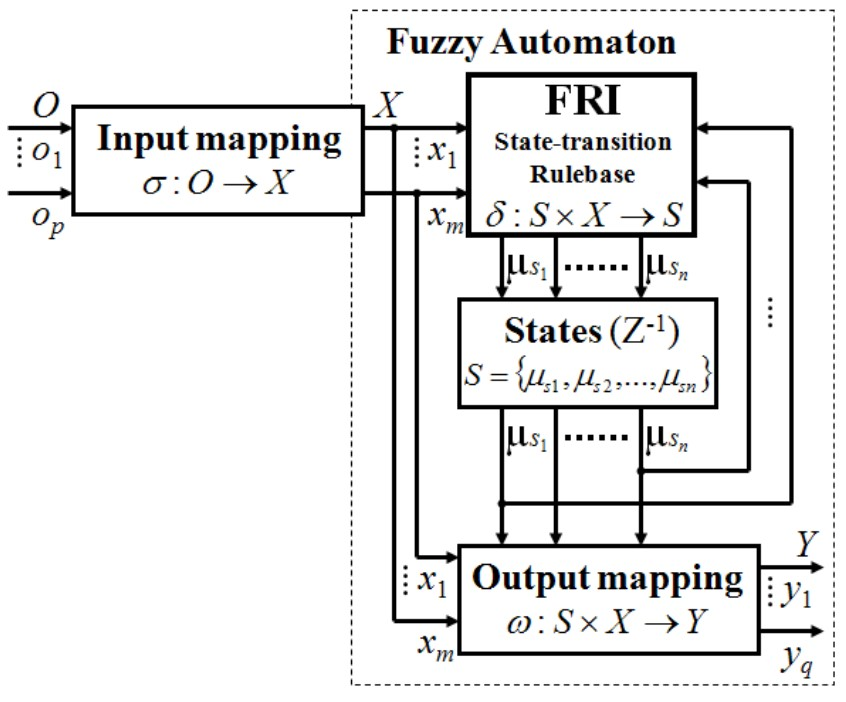
\includegraphics[width=0.6\textwidth]{images/fuzzy_automaton}
	\caption{Fuzzy Automaton}
\end{figure}

\Section{Fuzzy Behavior Description Language}
After having discussed in detail the needed prerequisites for greater understanding we can finally turn our attention to the main topic of this work, namely the language with which the aforementioned fuzzy behavior can be described. 


\SubSection{Motivation}
The language aims to provide an environment that enables the creation of programs utilizing fuzzy logic while requiring minimal to almost no prior knowledge in the field of programming. The target applications mainly entail those that delve into behavior control, as its name implies, and in order to facilitate the efficient development of such programs a higher level of abstraction is required leaving the specific implementations with regards to hardware constraints and fuzzy calculations to their respective layers of operation.

\SubSection{Language Specifications}
An easy to use language encompasses not just logical abstraction, but is also simple in terms of syntax.
An SQL-like syntax for verbosity and the lack of special characters or any complicated notation schemes makes it appeal to a wider audience than it would otherwise. The specifications for the grammar is provided below using the extended Backus-Naur form.

\begin{grammar}
<behavior> ::= universe+ rulebase+ [init]

<universe> ::= `universe' string [`description' string] symbol+ `end'

<symbol> ::= string number number

<rulebase> ::= `rulebase' string [`description' string] rules `end'

<rules> ::= rule+

<rule> ::= `rule' [`description' string] [`use'] string [`when' predicates] `end'

<predicates> ::= predicate (`and' predicate)*

<predicate> ::= string `is' string

<init> ::= `init' [`description' string] (string (string | number))+ `end'
\end{grammar}

For a more concise representation a railroad diagram of each element is also included \cite{pillerkovacs2015}.

\begin{figure}[!h]
	\centering
	\begin{subfigure}[b]{0.8\textwidth}
		\centering
        	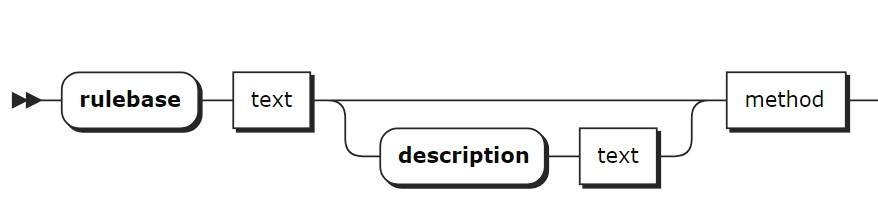
\includegraphics[width=0.8\textwidth]{images/rulebase_1}
		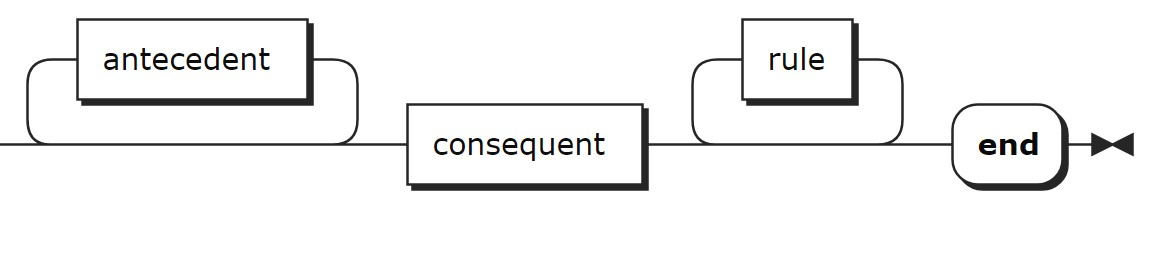
\includegraphics[width=0.8\textwidth]{images/rulebase_2}
        	\caption{Rulebase definition}
    \end{subfigure}
	
	\begin{subfigure}[b]{0.9\textwidth}
        	\centering
        	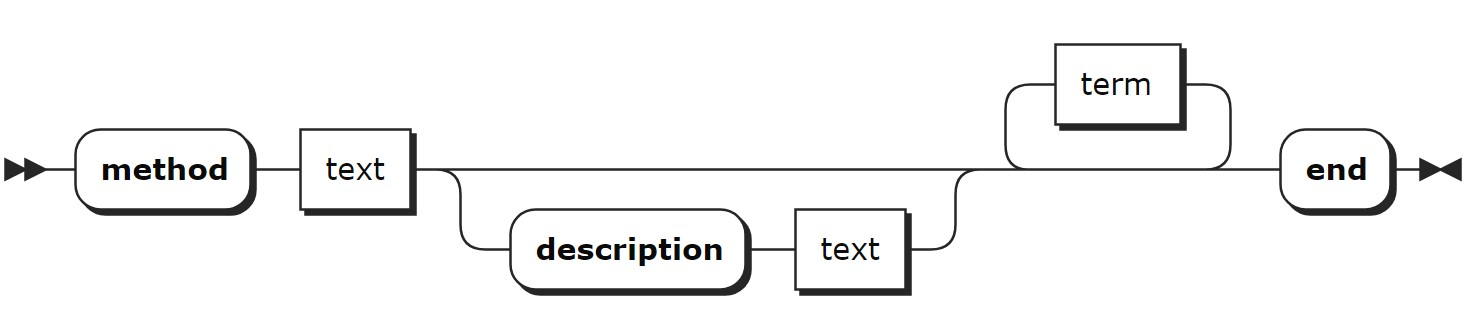
\includegraphics[width=0.8\textwidth]{images/method}
		\caption{Method definition}
    \end{subfigure}
    
    \begin{subfigure}[b]{0.9\textwidth}
        	\centering
        	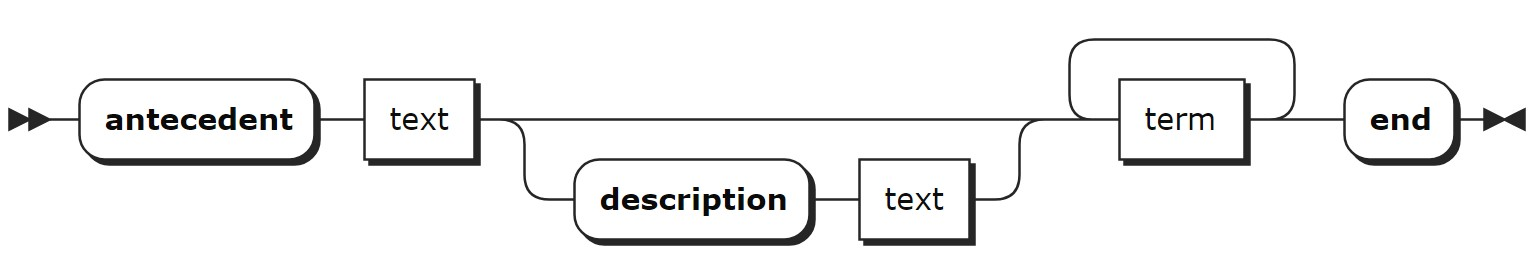
\includegraphics[width=0.8\textwidth]{images/antecedent}
		\caption{Antecedent definition}
    \end{subfigure}
    
    \begin{subfigure}[b]{0.9\textwidth}
        	\centering
        	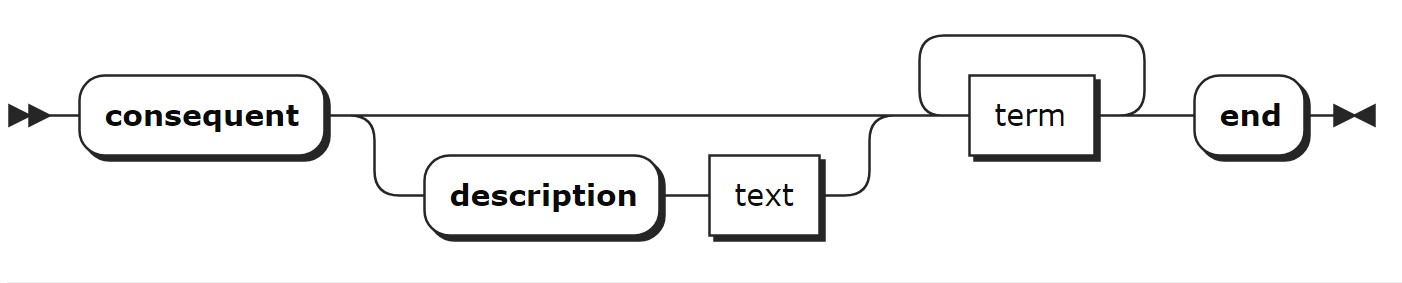
\includegraphics[width=0.8\textwidth]{images/consequent}
		\caption{Consequent definition}
    \end{subfigure}
    
	\caption{Syntax diagram of language elements}
\end{figure}

[Fix rule and term block]

The interpreter discussed in this work is based on a JavaScript implementation from the same paper \cite{pillerkovacs2015}.
